\documentclass[12pt,twoside]{report}

\usepackage[italian]{babel}
\usepackage[utf8]{inputenc}

\usepackage{graphicx}
\graphicspath{ {images/} }

\title{
  {La guerra fredda e le sue tensioni}\\
  {\large Cotugno-Carducci-GiovanniXXIII}
}

\author{Vincenzo Balducci}
\date{Giugno 2018}

\begin{document}

\maketitle

\tableofcontents

\chapter{Storia: La guerra fredda}
\section{I due blocchi}

\section{La crisi missilistica cubana}

\section{Il muro di Berlino}


\chapter{Inglese: JFK and Martin Luther King}
\section{John Fitzgerald Kennedy}
In 1960 John Fitzgerald Kennedy was elected president of the United States.

At forty-three he was the youngest man ever elected President of the USA, and the first one who was catholic.

He said to the Americans: <<Ask not what your countryu can do for you - Ask what you can do for your country>>.

\section{Martin Luther King}


\chapter{Scienze: L'atomo e la fissione nucleare}
\section{La struttura dell'atomo}
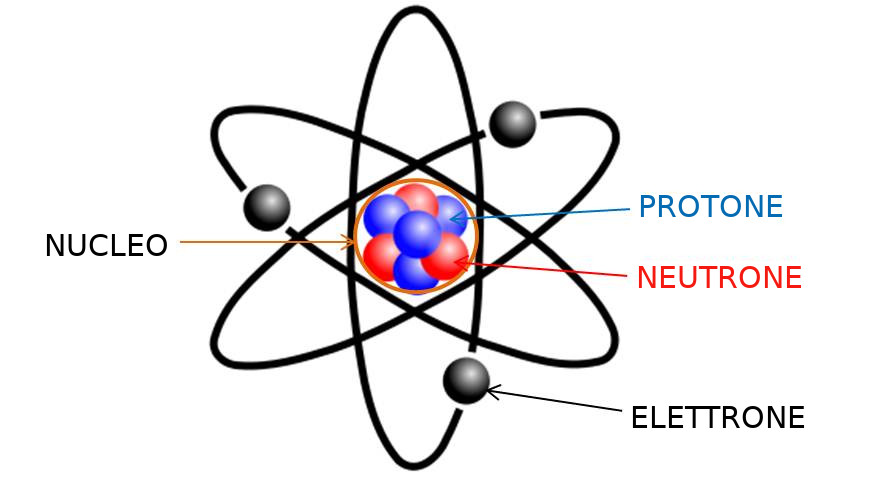
\includegraphics{atom.jpg}
L'atomo  è l'elemento più piccolo della materia ad avere proprietà chimiche. Esso è costituito da tre particelle subatomiche: i protoni e neutroni, che insieme formano il nucleo, e gli elettroni, che orbitano attorno ad esso lungo gli orbitali.

\section{L'uranio e la fissione nucleare}
L'uranio è un metallo pesante poco abbondante, ma largamente diffuso; se viene bombardato da un neutrone il suo nucleo si spezza in due nuclei più leggeri, il bario e il cripto. Da questa reazione, detta fissione nucleare, si libera una notevole quantità di energia e altri neutroni, che vanno a loro volta a colpire altri atomi di uranio. Si tratta di una reazione a catena, che una volta innescata continua da sola, liberando quantità sempre crescenti di energia.

Il primo dispositivo in grado di fare ciò fu ideato da Fermi ed entrò in funzione a Chicago il 2 dicembre 1942. Tale dispositivo venne chiamato pila atomica o reattore nucleare. E' formato da un'involucro di piombo nel cui interno si trova un cubo di grafite, sostanza che rallenta il movimento dei neutroni; nella grafite sono inserite delle barre di uranio alternate a barre di controllo fatte di boro e di cadmio, sostanze che regolano la quantità di neutroni assorbendoli se sono in eccesso. Sollevando o abbassando le barre di controllo è possibile innescare o bloccare la reazione a catena.


\chapter{Tecnica: Il circuito elettrico}
L’energia nucleare, nei tempi più recenti, viene soprattutto utilizzata per produrre energia elettrica.

La corrente elettrica è un flusso continuo di elettroni (cariche elettriche) che, attraverso un conduttore, si sposta ordinatamente da un punto di carica negativa (polo negativo) dove si è creato un eccesso di elettroni, a un altro punto di carica positiva (polo positivo) nel quale c’è una carenza di elettroni. Il flusso è costituito di cariche negative e perciò si muove verso il polo positivo: questa è la situazione reale.

L’intensità di corrente è la quantità di corrente che passa attraverso la sezione di un conduttore nell’unità di tempo ed è indicata con il simbolo I. Nel Sistema Internazionale, l’intensità della corrente elettrica si misura in ampere (simbolo A). Lo strumento di misura utilizzato è chiamato amperometro.

La corrente elettrica può essere:
\begin{itemize}
  \item continua se l’intensità e il verso rimangono costanti nel tempo;
  \item alternata se l’intensità e il verso cambiano periodicamente.
\end{itemize}

L’intensità di corrente elettrica è condizionata dalla differenza di carica elettrica esistente tra gli estremi del conduttore e dalla resistenza che il materiale di cui è fatto il conduttore oppone al suo passaggio. Questa differenza si chiama differenza di potenziale(d.d.p.) o in genere tensione elettrica , ed è indicata con il simbolo V. Tanto maggiore è la differenza di potenziale elettrico tanto maggiore è l’intensità di corrente a parità di resistenza. Nel SI, la differenza di potenziale si misura in volt (V) e lo strumento di misura utilizzato si chiama voltmetro.

I conduttori non trasportano la corrente tutti allo stesso modo ma offrono a essa una resistenza a farsi attraversare dalla corrente diversa. Il valore della resistenza dipende:
\begin{itemize}
  \item Dalle caratteristiche del materiale utilizzato per realizzare il conduttore;
  \item Dalla sezione del conduttore: la resistenza di un conduttore diminuisce all’aumentare della sua sezione.
\end{itemize}
La resistenza elettrica viene indicata con il simbolo R e si misura in ohm.


\chapter{Geografia: Cuba}
\section{Il territorio e il clima}
Cuba è la più vasta isola dei Caraibi; appartiene all'arcipelago delle Grandi Antille. E' costituita in gran parte da un'ampia {\bf pianura} calcarea. Le {\bf zone montuose} sono intervallate da ampie e fertili vallate. La {\bf costa} è generalmente bassa e paludosa. Al territorio cubano appartengono inoltre più di 1600 isole minori.

Il {\bf clima} è caldo e umido, ma mitigato dall'influenza del mare. Tra agosto e ottobre l'arcipelago è soggetto a cicloni provenienti da sud-ovest.

\section{Popolazione e città}
Oltre un terzo della popolazione è di origine bianca, per le consistenti migrazioni dall'Europa, sono presenti mulatti, neri e asiatici.

Oltre il 75\% dei cubani vive nelle città. L'Avana, la capitale, è la principale città dell'America centrale e importante centro di riferimento culturale di tutta l'America latina. Conserva il fascino dell'antico centro coloniale spagnolo, con palazzi e chiese; è inoltre un grande porto commerciale.

\section{Economia}
L'economia è sotto il controllo dello stato, governato da un regime comunista; negli ultimi anni, tuttavia, si sono introdotte riforme che lasciano maggiori spazi all'impresa privata e alle piccole aziende.

Settore tradizionalmente trainante dell'economia cubana, l'agricoltura conserva tuttora grande importanza. La canna da zucchero e il tabacco sono le coltivazioni principali. Discreti sono l'allevamento bovino e la pesca.

Le risorse del sottosuolo (petrolio, cobalto e rame) sono modeste.

L'industria comprende fabbriche per la trasformazione dei prodotti agricoli per la raffinazione del petrolio, la cui produzione resta però insufficiente.

Nel terziario è in espansione il turismo.


\chapter{Italiano: Soldati}
\section{La vita}
Giuseppe Ungaretti nacque ad Alessandria d’Egitto l’8 febbraio 1888 da genitori lucchesi emigrati in cerca di lavoro; studiò in una scuola di lingua francese della città egiziana.

Nel 1912 si trasferì a Parigi, dove frequentò l’Università della Sorbona e incontrò alcuni tra gli esponenti più importanti della cultura europea del tempo. Qui approfondì la conoscenza dei poeti simbolisti come Charles Baudelaire e Stephane Mallarmé, che esercitarono su di lui un’influenza fondamentale.

Nel 1914 si trasferì in Italia, dove, arruolatosi volontario come soldato semplice di fanteria, partecipò alla Prima guerra mondiale combattendo sul fronte del Carso.  Dall’esperienza diretta delle atrocità della guerra, drammaticamente vissute in prima persona, prese forma il primo nucleo della sua produzione poetica. Nacquero così le raccolte Il porto sepolto (1916) e Allegria di naufragi (1919); le poesie furono poi riunite nel volume L’Allegria (1931).

Al termine del conflitto, Giuseppe Ungaretti visse a Parigi per un anno, come corrispondente del giornale fondato da Benito Mussolini, "Il popolo d’Italia". L‘adesione al fascismo nasceva dall’ingenua fiducia nel rinnovamento economico e spirituale del popolo italiano che il regime prometteva attraverso la massiccia propaganda.

Tra il 1920 e il 1936 Giuseppe Ungaretti svolse un’intensa attività di giornalista e conferenziere, viaggiando molto in Italia e in Europa. Nel 1933 uscì la raccolta Sentimento del Tempo.

Nel 1936 Giuseppe Ungaretti accettò la cattedra di Lingua e letteratura italiana presso l’Università di San Paolo, in Brasile, dove andò a vivere con la moglie e i due figli. Qui lo colpirono due gravi lutti familiari: la morte del fratello Costantino e quella del figlio Antonietto, prematuramente scomparso all’età di soli dieci anni.

Il ritorno in Italia nel 1942 coincise con la Seconda guerra mondiale. Alla tragedia privata si sovrappose così quella pubblica e questo duplice dramma ispirò la raccolta emblematicamente intitolata Il Dolore (1947). Fu nominato Accademico d’Italia e ottenne "per chiara fama" la cattedra di Letteratura italiana moderna e contemporanea all’Università di Roma.

Pubblicò le raccolte La Terra Promessa (1950), Un Grido e Paesaggi (1952), Il taccuino del vecchio (1960), Dialogo (1968) e le traduzioni di alcuni importanti autori di lingua inglese, francese, spagnola.

Nel 1970 fu colto da malore durante un viaggio negli Stati Uniti e, rientrato in Italia, morì a Milano, il 2 giugno, per broncopolmonite, all’età di ottantadue anni.

\section{Soldati}

\begin{verse}
  Si sta come \\
  d'autunno \\
  sugli alberi \\
  le foglie
\end{verse}

La lirica è di Giuseppe Ungaretti , tratta da Vita di un uomo.

Questa poesia è composta da solamente un periodo costituito da quattro versi senza rime e in più brevissimi, ma che comunicano con la loro essenzialità sintattica significati molto più profondi.

Sarebbe difficile comprendere il significato della lirica senza leggere il titolo : “Soldati”.

Troviamo già all’inizio una similitudine e questo è il primo termine di paragone. La lirica esprime quel filo invisibile tra la vita e la morte in cui si trovano i soldati, cioè come foglie sugli alberi in autunno che cadono con un soffio di vento: la morte. Come le foglie nascono e muoiono, allo stesso modo fanno gli uomini.

E’ significativo l’enjambement dopo il come che rende ancora meglio l’idea di stabilità comunicata dal verbo stare.

In questa lirica, come in parecchie altre riferite alla guerra (Risvegli, Veglia, San Martino del Carso) Ungaretti esprime lo stato d’animo in cui ci si trova spesso in guerra, in questo caso la tensione della morte imminente.

Questo breve componimento di Giuseppe Ungaretti  si trova nella raccolta L’ Allegria, più specificatamente nella parte dell’ opera intitolata Girovago. Questa poesia è formata un’unica similitudine, soldati/foglie; dal punto di vista metrico, la lirica presenta due settenari divisi in quattro versi e un enjambement tra il primo e il secondo verso.

Leggendo il testo notiamo subito come quest’ultimo, insieme a moltissimi altri presenti nella medesima raccolta, si riferisca alla guerra, e sia attraversato da un presagio di morte.

Perché, dunque, chiamare L’allegria una raccolta di poesie in cui prevalgono tali temi?

Ungaretti spiega come il sentimento dell’allegria, in questo caso, scaturisca nell’attimo in cui l’uomo realizza di essere scampato alla morte. L’esperienza diretta che il poeta fa della guerra durante il primo conflitto mondiale, la quotidiana tensione verso la vita nell’atto pratico della sopravvivenza, porta al culmine tale sentimento. Soldati rientra certamente in questo filone tematico. Composto nel 1918 mentre Ungaretti si trovava in trincea nel bosco di Courton, esprime il dramma e la precarietà del momento storico e della condizione umana. I soldati vengono qui paragonati a foglie autunnali che, ancora appese agli alberi, procedono inevitabilmente verso la caduta e la morte, vittime dello scorrere del tempo.

Al termine “soldati” è però facilmente sostituibile quello di uomini, e alla guerra è applicabile la più ampia nozione di vita. Così ci rendiamo conto come non siano solo i militari al fronte a vivere una condizione precaria e incerta, ma come sia la natura stessa dell’essere umano a dover fare i conti con la propria finitudine.

Il parallelismo tra uomo e foglie, immagine molto riuscita, non è una scelta letteraria innovativa operata da Ungaretti, ma possiamo ritrovarla in testi poetici anche molto antichi, ad esempio nell’Iliade.



\chapter{Spagnolo: Picasso}
\begin{center}
  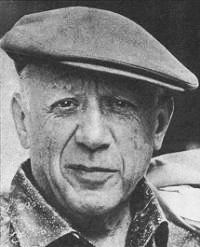
\includegraphics[width=0.55\textwidth]{pablo.jpg}
\end{center}

Pablo Picasso fue un pintor español creador del cubismo. Su padre fue profesor en la academia de bellas artes y ayudò su hijo con la pintura.
Se conoce como periodo azul de picasso al que discurre entre 1901 hasta 1904 y tiene su origen en el suicidio de su amigo que lo dejò lleno de dolor y tristeza.
En el 1905 el pasò de la epoca azul a la denominada epoca rosa que se destinsue por sus colores pastel y tonos càlidos, con lineas delicadas.
Con las señoritas de aviñon como punto de partida Picasso acabò formulando el cubismo.
En el 1937 se produjò el brutal bombardeo de la localidad de Guernica por parte de la Alemania.
Picasso se inspirò en este hecho para la creaciòn de una de sus obras mas famosas.
El cuadro simboliza dodo ul horror de la guerra y la tragedia de la muerte de muchas victimas inocentes.
En 1973 , a la edad de 91 años, muriò en Francia.


\chapter{Arte: la Guernica}
\section{Il cubismo}
Il cubismo fu una delle correnti più innovative del '900. Nacque a Parigi intorno al 1907 per opera di Pablo Picasso e Georges Braque. Come punto di riferimento il cubismo prende spunto dall'attenta osservazione della pittura di Cézanne e del suo modo di rappresentare la natura scomponendola in forme geometriche elementari e sia sulla conoscenza dell'arte primitiva.

Il soggetto rappresentato è visto da più punti di osservazione contemporaneamente; l'immagine viene smontata nelle sue parti essenziali, analizzata dalle diverse angolazioni e poi riassemblata. In questo modo i cubisti introdussero il concetto di quarta dimensione: il tempo dell'osservazione.

Gli studiosi individuarono tre fasi del movimento cubista:
\begin{itemize}
  \item Cubismo formativo, caratterizzato da una progressiva deformazione e semplificazione dei volumi;
  \item Cubismo analitico, che si caratterizza per la frantumazione del soggetto in elementi così piccoli da renderne difficile il riconoscimento;
  \item Cubismo sintetico, si caratterizza per una rappresentazione più diretta e immediata della realtà dando spazio nei quadri cubisti a scritte e ai "papier collès", ovvero frammenti, incollati sulla tela, di giornali, carte da parati, carte da gioco e frammenti di legno. Il cubismo sintetico rivoluziona il concetto stesso di quadro portandolo ad essere esso stesso "realtà" e non "la rappresentazione della realtà"
\end{itemize}

\section{Pablo Picasso}
Nato a Malaga, in Spagna, nel 1881 Pablo Picasso si trasferì nel 1900 a Parigi dove entrò in contatto con l'ambiente intellettuale.

Le sue prime opere hanno per soggetto la vita degli emarginati e la vita del circo; la svolta si ha nel 1907 qunado la sia opera Les Demoisseles d'Avignon segna la nascita del cubismo. Durante la sua esistenza realizzò un gran numero di opere utilizzando diverse tecniche e stili. La figura di Picasso è importante anche per l'impegno civile dimostrato con il celebre dipinto Guernica.

\section{La Guernica}
Guernica era una piccola città della Spagna rasa al suolo nel 1937 da un bombardamento tedesco. Picasso decise di commemorare la strage dipingendo una grande tela per l'Esposizione Universale di Parigi del 1937. L'opera si basa su una costruzione piramidale in cima alla quale si trova un cavallo ferito che simboleggia la sofferenza del popolo spagnolo. Al vertice della composizione ci sono una luce elettrica e una lampada a olio, simboli della verità che trionfa sulla menzogna; sulla sinistra del quadro c'è un toro simbolo di forza. In basso a sinistra c'è l'immagine di una donna straziata dal dolore per la perdita del figlio; in alto a destra è raffigurata una donna con le braccia verso il cielo mentre la sua casa prende fuoco; in basso giace un soldato che impugna una spada sulla quale è nato un fiore simbolo di speranza.

Nella sua opera Picasso non vuole solo rappresentare la guerra di Guernica ma rappresenta la distruzione a cui porta il regime totalitario sollecitando tutti gli intellettuali e le forze popolari a schierarsi in difesa della libertà.


\chapter{Musica: Il jazz}
Il Jazz nacque a New Orleans da una commistione fra blues e sonorità di influenza europea ed africana, e conobbe la sua maggiore popolarità soprattutto a partire dagli anni '20.

Durante gli anni' 30 dal jazz si sviluppò un nuovo genere musicale, lo swing, caratterizzato da una spensieratezza e da uno ritmo "dondolante" (lo swing, appunto). Questo genere musicale divenne molto popolare durante gli anni della Seconda Guerra Mondiale e questo fu l'unico momento storico in cui il jazz, tradizionalmente considerato come musica "colta", riuscì a raggiungere le masse, conoscendo una diffusione che mai si era avuta e che mai più si è ripetuta.

La musica jazz e la Seconda Guerra Mondiale ebbero una forte e reciproca influenza: la rivista americana "Down Beat" pubblicò queste parole "I musicisti oggi, non sono soltanto suonatori di jazz, loro sono i soldati della musica", questo perché il jazz contribuì a tenere alto il morale dei soldati impegnati sul fronte di guerra e, nello stesso tempo, fu di conforto per i loro cari rimasti ad attenderli in patria. La musica e i pochi divertimenti che i soldati si concedevano al fronte erano forieri di cari ricordi che aiutavano e motivavano i giovani ad impegnarsi per riuscire a tornare a casa il più presto possibile. Inoltre la musica era certamente utile per distrarsi e trovare un momento di distacco dagli orrori che venivano vissuti quotidianamente sui campi di battaglia.

In quegli anni molti musicisti jazz si arruolarono volontariamente nell'esercito, altri, invece, portarono i loro concerti negli Stati Uniti o, quando possibile, anche all'estero, contribuendo a diffondere i valori americani nel mondo. Se però il jazz ebbe un impatto importante sulla guerra, anche la guerra influì sul genere musicale allora più popolare in America.

Intanto, a causa dei razionamenti della benzina, viaggiare era diventato più difficoltoso: c'erano meno autobus a disposizioni delle orchestre e i treni, spesso, erano occupati dai soldati che partivano o tornavano dall'Europa. In quegli anni, inoltre, una forte tassa sugli intrattenimenti serali decretò la chiusura di molte sale da ballo americane che non riuscivano più a sostenere i costi di gestione, in un momento economicamente già piuttosto difficile. In più, nel 1942, la Federazione Americana dei Musicisti impose un divieto di registrazione agli artisti(il Recording Ban), almeno fino a quando le case discografiche non si fossero impegnate nel pagamento dei diritti d'autore per le canzoni suonate alla radio e nei juke-box.

Fu in questo periodo abbastanza difficile della musica jazz, che si impose un nuovo genere: il bebop. Dizzie Gillespie e Charlie Parker ne furono gli iniziatori, ben presto seguiti da molti altri musicisti. Caratteristica del bebop sono i tempi molto veloci, le dissonanze armoniche e l'improvvisazione, vera anima di questo genere musicale astratto e ribelle.


\chapter{Scienze motorie: le olimpiadi dell'80}
Vincere, vincere, vincere. Che sia in americano o in russo, questo è stato l’imperativo degli atleti dei due blocchi durante le Olimpiadi del dopoguerra.

Helsinki 1952, quindicesima Olimpiade

A Helsinki Stalin decide di far partecipare anche la sua nazione, ma la Finlandia era la stessa terra che aveva combattuto contro l’Armata Rossa e inoltre era oggetto da tempo delle mire espansionistiche russe: con l’avvicinarsi dei Giochi quindi le tensioni politiche si moltiplicano sempre di più.

L’attrito si manifesta quando viene chiesto ai sovietici di far passare la fiaccola attraverso i Paesi Baltici, permesso che la Russia nega, costringendo l’organizzazione finlandese a cambiare il percorso attraverso i Paesi Scandinavi.

Un altro momento cruciale avviene pochi giorni prima dell’inizio della manifestazione quando le Autorità di Mosca avanzano la pretesa di porre come base per i loro atleti Leningrado e non la capitale finlandese. Alla fine le due Nazioni trovano un compromesso: gli atleti russi avrebbero avuto un villaggio olimpico separato dagli altri.

Le Olimpiadi di Helsinki segnano non solo l’esordio della Russia ma anche la riammissione della Germania e del Giappone.

La congregazione sovietica, alla sua prima partecipazione, riesce a portare in patria 71 medaglie contro le 76 degli USA.


\chapter{Religione: Lo stato senza dio}
/section{Dio non esiste}


\end{document}
